%
% حق نشر 1390-1402 دانش پژوهان ققنوس
% حقوق این اثر محفوظ است.
% 
% استفاده مجدد از متن و یا نتایج این اثر در هر شکل غیر قانونی است مگر اینکه متن حق
% نشر بالا در ابتدای تمامی مستندهای و یا برنامه‌های به دست آمده از این اثر
% بازنویسی شود. این کار باید برای تمامی مستندها، متنهای تبلیغاتی برنامه‌های
% کاربردی و سایر مواردی که از این اثر به دست می‌آید مندرج شده و در قسمت تقدیر از
% صاحب این اثر نام برده شود.
% 
% نام گروه دانش پژوهان ققنوس ممکن است در محصولات دست آمده شده از این اثر درج
% نشود که در این حالت با مطالبی که در بالا اورده شده در تضاد نیست. برای اطلاع
% بیشتر در مورد حق نشر آدرس زیر مراجعه کنید:
% 
% http://dpq.co.ir/licence
%
\section{برگه‌ها}

یک برگه عبارت است از یک مستند کاملا سازماندهی شده که به صورت مستقیم با هیچ یک از
موجودیت‌های یک سیستم در ارتباط نیست. به بیان دیگر یک برگه گرچه به عنوان قسمتی از
مستند فنی در نظر گرفته می شود اما به صورت مستقیم هیچ یک از موجودیت‌های سیستم
مانند کلاسها، فضاهای نام و غیره را تشریح نمی‌کند.

مستندهای که مانند مستند نصب و راه اندازی یک سیستم، که به صورت مستقیم مربوط به
قسمتی خاص از یک سیستم نمی‌شود ولی در عین حال یک مستند فنی بسیار مهم در نظر گرفته
می‌شود، با استفاده از برگه‌ها ایجاد می‌شوند.

گرچه در فرآیند مستند فنی، در ساختارهای متفاوت، دید متفاوتی نسبت به یک برگه وجود
دارد اما در حالت کلی می‌توان یک برگه را معادل با یک گفتار در نظر گرفته که به
توصیف و تشریح جنبه‌ای خاص از سیستم می‌پردازد. در حالت کلی یک برگه به صورت زیر در
مستند فنی ایجاد می‌شود:


\begin{latin}
\lstset{language=C++}  
\begin{lstlisting}[frame=single] 
\page <name> (title)
\end{lstlisting}
\end{latin}

که در آن \lr{<name>} یک شناسه و \lr{(title)} عنوان مورد نظر برای برگه است. عنوان
یک عبارت است که برای نمایش یک برگه به کار می‌رود در حالی که شناسه تنها برای
ایجاد پیوند به هر برگه مورد استفاده قرار می‌گیرد. برخلاف عنوان که می‌تواند هر
عبارتی باشد شناسه تنها از حروف نوشتاری و عدد ایجاد می‌شود که شامل هیچ فاصله‌ای
نیست.

\begin{note}
شناسه ترکیبی از حروف و ارقام است. در برخی از سیستم‌های عامل مانند لینوکس و
یونیکس، حروف بزرگ و کوچک با یکدیگر تفاوت دارند در حالی که در برخی دیگر اینگونه
نیست. از این رو ممکن است برخی از توسعه دهندگان از حروف بزرگ و یا ترکیب آن با
حروف کوچک برای ایجاد شناسه استفاده کنند (برای نمونه \lr{MyPage01}). 
\\%FIXME: maso 1391 این قسمت باید به دو پاراگراف تبدیل شود.
گرچه استفاده از حروف بزرگ و کوچک در نامگذاری برگه‌ها مخصوصا زمانی که اندازه
مستند بزرگ است، می‌تواند مفید باشد اما با مشکل‌های نیز روبرو است. برای نمونه در
ایجاد مستند فنی نهای بر اساس قالب خاص، مانند \lr{HTML} پرونده‌هایی هم نام با
شناسه‌های برگه‌ها ایجاد می‌شود از این رو در سیستم عامل‌هایی مانند ویندوز، که در
آنها تفاوتی میان حروف بزرگ و کوچک نیست، مشکلهایی در خروجی ایجاد شده به وجود
می‌اید. از این رو بهتر است که تمام شناسه‌ها را تنها با استفاده از حروف کوچک
ایجاد کرد.
\end{note}

برای نمونه قطعه مستند زیر را در نظر بگیرید:
\begin{latin}
\lstset{language=C++}  
\begin{lstlisting}[frame=single] 
/**
 * \page pageinstall Install
 * 
 * Installation (or setup) of a computer program (including device drivers and plugins),
 * is the act of making the program ready for execution. Because the process varies
 * for each program and each computer, programs (including operating systems) often
 * come with an installer, a specialized program responsible for doing whatever is
 * needed for their installation.
 */
\end{lstlisting}
\end{latin}

در این نمونه یک برگه با عنوان \lr{Install} ایجاد شده است که با استفاده از شناسه
\lr{pageinstall} شناخته می‌شود. متن هر برگه نیز می‌تواند با استفاده از تمام
برچسب‌های مورد حمایت در \lr{Doxygen} ایجاد شود.


\subsection{بخش بندی برگه}

بخش بندی عبارت از فرآیندی که در آن یک مستند بزرگ به صورت منطقی به صورت تکه‌های
مستند کوتاه در یک ساختار سلسله مراتبی سازماندهی می‌شوند. امروزه بخش بندی کردن
مستندها انقدر مرسوم است که حتی یک مستند چند صفحه‌ای هم بخش بندی می‌شود. برای
نمونه یک کتاب را در نظر بگیرید که در آن موضوع‌های متفاوت با استفاده از فصل‌ها و
گفتارها جدا شده‌اند. با وجود دسته بندی مطالب یک بر اساس موضوع آنها در گفتارهای
متفاوت، خود گفتارها نیز باز به صورت بخش و زیر بخش سازماندهای می‌شوند.

سازماندهی کردن یک مستد بزرگ با استفاده از بخش بندی نه تنها مطالعه و درک آن را
راحتر می‌کند بلکه فرآیند توسعه و نگه داری آن را هم نیز بهبود می‌بخشد. تصور اینکه
یک نویسنده کتابی چند صد صفحه‌ای را بدون تقسیم بندی و سازماندهی کردن بتواند ایجاد
کند انقدر دشوار است که می‌توان آن را معادل با ایجاد یک سیستم بدون معماری در نظر
گرفت. می‌توان گفت بخش بندی در حقیقت ایجاد یک معماری برای یک مستند بزرگ است از
این رو در توسعه و به کار گیری آن بسیار موثر خواهد بود.

از سویی ایجاد یک مستند ساختارمند استفاده از آن را نیز آسان می‌کند. امروزه تمام
کتاب‌ها و مستندها از تکنیک‌های مانند فهرست گذاری استفاده می‌کنند که در آن  یک
فهرست از تمام موضوع‌ها و ارجاع به آن ( مانند شماره صفح) وجود دارد، استفاده
می‌کنند. ایجاد یک فهرست مناسب برای یک مستند بسیار حیاطی است. اما ایجاد این فهرست
به صورت دستی بسیار زمانگیر است و در محیط‌هایی که مستند به سرعت تغییر می‌کند یک
ایراد اساسی به شمار می‌آید. با این وجود اگر از تکنیک‌های مناسبی برای ایجاد
بخش‌ها استفاده شود به سادگی می‌توان فهرست‌ها را به صورت خودکار ایجاد کرد و از
هزینه‌های توسعه مستند کاست.

یک مستند را می‌توان به صورت یک درخت در نظر گرفته که به صورت موضوعی ایجاد شده
است. برای نمونه ساختار درختی در شکل 
\ref{images/write/grouping/section-tree} را در نظر بگیرید. در این شکل (که قسمتی
از ساختار سلسله مراتبی این کتاب را نمایش می‌دهد) یک ساختار درختی نمایش داده شده
است که سازمان کلی یک مستند را نمایش می‌دهد. این ساختار از بالاترین سطح با
استفاده از فصل، گفتار، بخش، زیر بخش  و \ldots در یک مستند حقیقی پیاده سازی
می‌شود.

\begin{figure}
	\centering
	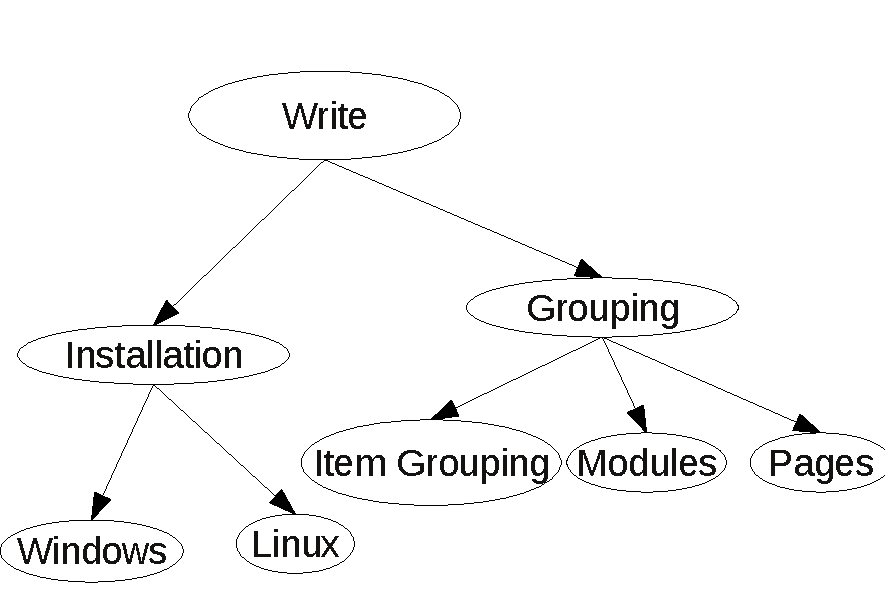
\includegraphics[width=0.75\textwidth]{images/write/grouping/section-tree}
	\caption[ساختار سلسله مراتبی یک مستند]{
		همان گونه که در این شکل نمایش داده شده است یک مستند را می‌توان با استفاده
		از یک ساختار سلسله مراتبی که به صورت یک درخت قابل بیان است، سازماندهی کرد.
	}
	\label{images/write/grouping/section-tree}
\end{figure}

ساختارهای متفاوت نشر، روش‌هایی را برای پیاده سازی این ساختار سلسله مراتبی
پیشنهاد می‌کنند. برای نمونه \lr{HTML} که به عنوان پر کاربرد ترین ساختار متنی در
شبکه جهانی، با استفاده از مفاهیم سرآیندها این ساختار را پیاده سازی می‌کند. در
این ساختار بالاترین سطح یک مستند با استفاده از برچسب \lr{<h1>\ldots</h1>} ایجاد
می‌شود. سطح‌های بعدی مستند که می‌تواند به صورت تود در تو مورد استفاده قرار گیرد
با استفاده از برچسب‌های \lr{<h2>\ldots</h2>}, \ldots و \lr{<h9>\ldots</h9>}
ایجاد می‌شود. از این رو ساختار معرفی شده در
شکل\ref{images/write/grouping/section-tree} به صورت زیر قابل بیان است:

\begin{latin}
\lstset{language=HTML}  
\begin{lstlisting}[frame=single] 
<h1>Writer</h1>
	<h2>Grouping</h2>
		<h3>Pages</h3>
		<h3>Modules</h3>
		<h3>Item Grouping</h3>
	<h2>Installation</h2>
		<h3>Linux</h3>
		<h3>Windows</h3>
\end{lstlisting}
\end{latin}

امکان ایجاد ساختار سلسله مراتبی در مستندهای تکنیکی نیز می‌تواند بسیار مفید باشد
مخصوصا زمانی که مستندهای تکنیکی به مرور زمان و به سرعت تغییر می‌کنند و یا اینکه
اندازه مستندهای ایجاد شده بزرگ باشد. در این بخش برچسب‌های تعریف شده در
استانداردهای \lr{Doxygen} که در ایجاد این ساختار سلسله مراتبی مورد استفاده قرار
می‌گیرد را به صورت کامل مورد بررسی قرار خواهیم داد.

\begin{note}
ساختارهای سلسله مراتبی معرفی شده در این بخش نه تنها قابل استفاده در برگه‌ها
هستند بلکه می‌توان آنها را در هر قسمت دیگر از مستند نیز به کار برد.
\end{note}

% TODO: مصطفی ۱۳۹۱: تعیین منبع برای نوشتن استاندار
% در نوشتن استاندارد از چهار سطح استفاده می‌شود که باید منبع آن را ذکر کرد. فکر
% کنم از استانداردهای ISO برای مستند کاربری بود.
\begin{info}
بر اساس استانداردهای موجود در ایجاد مستندها، ایجاد ساختار سلسله مراتبی در متن
مستند، با بیش از چهار سطح مناسب نیست.  از این رو در بسیاری از ابزارهای مستند
سازی مانند \lr{Doxygen} تنها امکان ایجاد سلسله مراتبی با کمتر از چهار سطح فراهم
شده است.
\end{info}

\paragraph{بخش}

بخش\LTRfootnote{Section} بالاترین سطح را در ساختار سلسله مراتبی مستند دارد.
در حالت کلی یک بخش با استفاده از برچسب \lr{\\Section} و به صورت زیر ایجاد
می‌شود:


\begin{C++}
\section <section-name> (section title)
\end{C++}

این برچسب شامل دو پارامتر است که عبارت اند از \lr{<section-name>} و \lr{Section
title}. نام به صورت یک شناسه در نظر گرفته می‌شود که با استفاده از آن می‌توان یک
بخش را به صورت منحصر به فرد آدرس دهی کرد. این شناسه تنها باید با استفاده از حروف
و ارقام ایجاد شده و شامل هیچ فاصله‌ای نباشد. عنوان یک بخش نیز یک عبارت است که
برای نمایش بخش مورد استفاده قرار می‌گیرد.

\begin{warning}
از این برچسب تنها در یک برگه (یا یک بسته مستند) استفاده می شود و نمی‌تواند در
سطوح پایین تر سلسله مراتبی مستند مورد استفاده قرار گیرد.
\end{warning}
    

\paragraph{زیر بخش}

زیر بخش\LTRfootnote{Subsection} دومین سطح از ساختار سلسله مراتبی مستندهای فنی را
ایجاد می‌کند. این سطح از مستند با استفاده از برچسب \lr{subsection} ایجاد می‌شود
که در حالت کلی به صورت زیر است:

\begin{C++}
\subsection <subsection-name> (subsection title)
\end{C++}

این برچسب نیز شامل دو پارامتر است که عبارت اند از \lr{<subsection-name>} و
\lr{Subsection title}. نام به صورت یک شناسه در نظر گرفته می‌شود که بر اساس قواعد
تعیین شناسه (یعنی تنها با استفاده از حروف و ارقام ایجاد شده و شامل هیچ فاصله‌ای
نباشد) ایجاد شده و با استفاده از آن می‌توان یک زیر بخش را به صورت منحصر به فرد
آدرس دهی کرد.
. عنوان یک زیر بخش نیز یک عبارت است که برای نمایش زیر بخش مورد استفاده قرار
می‌گیرد.

\begin{warning}
یک زیر بخش تنها باید در یک بخش مورد استفاده قرار گیرد و استفاده آن در هر قسمت
دیگر مجاز نمی باشد.
\end{warning}

زیر بخش، در ساختار سلسله مراتبی مستند به عنوان یک قسمت از بخشی در نظر گرفته
می‌شود که پیش از زیر بخش مورد نظر ظاهر شده است. برای نمونه قطعه مستند زیر را در
نظر بگیرید:

\begin{latin}
\lstset{language=C++}  
\begin{lstlisting}[frame=single] 
/**
 * ...
 * \section section1 Writer
 * ...
 * \section section2 Appendex
 * ...
 * \subsection subsection1 Performance
 * ...
 */
\end{lstlisting}
\end{latin}

در این تکه مستند دو بخش و یک زیر بخش ایجاد شده است. زیر بخش ایجاد شده با شناسه
\lr{subsection1} به نزدیکترین بخشی که پیش از آن تعریف شده است تعلق دارد از این
رو این زیر بخش به عنوان یک زیر بخش از بخش \lr{section2} در نظر گرفته می‌شود.

\paragraph{زیر زیر بخش}

سومین سطح در ساختار سلسله مراتبی مستندها را زیر زیر
بخش\LTRfootnote{Subsubsection} ایجاد می‌کند. برای ایجاد یک زیر زیر بخش در مستند
فنی از برچسب \lr{subsubsection} استفاده می‌شود که در حالت کلی به فرم زیر است:

\begin{latin}
\lstset{language=C++}  
\begin{lstlisting}[frame=single] 
\subsubsection <subsubsection-name> (subsubsection title)
\end{lstlisting}
\end{latin}

در اینجا نیز همانند برچسب زیر بخش، از دو پارامتر استفاده می‌شود که عبارت‌اند از:
\lr{subsubsection-name} و \lr{subsubsection-title}. این پارامترها که به ترتیب
شناسه و عنوان زیر زیر بخش را ایجاد می‌کنند، از همان قواعدی که برای زیر بخش بیان
شده است پیروی می‌کنند.

\begin{warning}
شناسه‌هایی که برای یک بخش، زیر بخش , \ldots در نظر گرفته می‌شود باید در حالت کلی
منحصر به فرد باشد. به بیان دیگر زمانی که برای یک بخش از یک شناسه استفاده می شود
نباید شناسه مورد استفاده را برای هیچ بخش، زیر بخش، و غیر به کار برد.
\end{warning}

استفاده از یک زیر زیر بخش تنها در یک زیر بخش مجاز است. هر زیر زیر بخش به عنوان
یک زیر بخش از نزدیکترین زیر بخشی در نظر گرفته می‌شود که پیش از آن تعریف شده
باشد. تکه مستند زیر را در نظر بگیرید:

\begin{latin}
\lstset{language=C++}  
\begin{lstlisting}[frame=single] 
/**
 * ...
 * \section section1 Writer
 * ...
 * \subsection subsection11 Installation
 * ...
 * \subsubsection subsubsection111 Linux
 * \subsubsection subsubsection112 Windows
 * ...
 * \subsection subsection12 Grouping
 * ...
 * \subsubsection subsubsection121 Pages
 * \subsubsection subsubsection122 Modules
 * \subsubsection subsubsection123 Pages
 * ...
 * \section section2 Appendex
 * ...
 * \subsection subsection1 Performance
 * ...
 */
\end{lstlisting}
\end{latin}

در این قطعه مستند سه زیر بخش با شناسه‌های \lr{subsubsection12x} ایجاد شده است.
از آنجا که نزدیکترین زیر بخش تعریف شده قبل از این سه زیر زیر بخش، زیر بخش با
شناسه \lr{subsection12} است، هر سه این زیر زیر بخش ها در این زیر بخش قرار خواهند
گرفت. نمونه بالا معادل با ساختار سلسله مراتبی است که در شکل
\label{write-grouping-pages-section-tree} نمایش داده شده است.
 
    
\paragraph{پاراگراف}

چهارمین سطح از ساختار سلسله مراتبی پاراگراف\LTRfootnote{Paragraph} است که در
حقیقت آخرین سطح از ساختار سلسله مراتبی در نظر گرفته می‌شود. هر تکه متن نوشته شده
در مستند به صورت یک پاراگراف در نظر گرفته می‌شود اما با این حال می‌توان با
استفاده از برچسب \lr{paragraph} یک پاراگراف را نام گذاری کرد. نام گذاری کردن یک
پاراگراف زمانی که نیاز به ارجا به متن آن باشد بسیار مفید است. ایجاد یک پاراگراف
در حالت کلی به صورت زیر است:

\begin{latin}
\lstset{language=C++}  
\begin{lstlisting}[frame=single] 
\paragraph <paragraph-name> (paragraph title)
\end{lstlisting}
\end{latin}

این برچسب نیز مانند برچسب های پیش از دو پارامتر به نام‌های \lr{paragraph-name} و
\lr{paragraph-title} استفاده می‌کند که بر اساس قواعد تعریف شده در برچسب‌های
پیشنین، تعیین می‌شوند. تفاوت اساسی که میان پاراگراف با تمام برچسب‌هایی که پیش از
برای استفاده در ساختارهای سلسله مراتبی بیان شده است، عدم شماره گزاری شدن این
برچسب است. در خروجی ایجاد شده برای یک پاراگراف، عنوان به صورت برجسته در ابتدای
سطر نوشته شده و متن موجود در ادامه آن آورده می‌شود.

\begin{note}
هر پاراگراف به نزدیکترین برچسب تعریف شده قبل از آن تعلق
دارد که در ساختارهای سلسله مراتبی مورد استفاده قرار می‌گیرد. به بیان دیگر این
برچسب به عنوان زیر بخشی از برگه، بخش، زیربخش، و یا زیر زیر بخشی تعلق دارد که پیش
از آن تعریف شده است.
\end{note}
    

\subsection{\lr{mainpage}}

همواره در قالب‌های متفاوت خروجی، از یک برگه به عنوان برگه نخست در مستند استفاده
می‌شود. گرچه برگه نخست نیز همانند دیگر برگه‌ها ایجاد و ویرایش می‌شود اما برخلاف
برگه‌های دیگر با استفاده از برچسب \lr{mainpage} ایجاد می‌شود. ساختار کلی این
دستور به صورت زیر استک

\begin{latin}
\lstset{language=C++}  
\begin{lstlisting}[frame=single] 
\mainpage [(title)]
\end{lstlisting}
\end{latin}

همانگونه که پیش از این نیز اشاره شده، برای ایجاد یک برگه از دو پارامتر استفاده
می‌شد که عبارت بودند از: عنوان و شناسه. برگه نخست تنها برگه‌ای است که تنها یک
پارامتر دارد و آن هم عنوان است. از آنجا که این برگه همواره در کل مستند فنی یکتا
است، یک شناسه پیش فرض به صورت \lr{index} برای آن در نظر گرفته می‌شود بنابر این
برچسب \lr{mainpage} معادل با برچسب زیر است:

\begin{latin}
\lstset{language=C++}  
\begin{lstlisting}[frame=single] 
\page index [(title)]
\end{lstlisting}
\end{latin}

\begin{warning}
از آنجا که شناسه \lr{index} به صورت پیش فرض برای برگه نخست در نظر گرفته شده است،
استفاده از این شناسه برای دیگر برگه‌های یا بخش‌های مستند مجاز نیست و منجر به
بروز مشکل در خروجی تولید شده می شود.
\end{warning}

به عنوان نمونه در مستند زیر برگه نخست مستند ایجاد شده است. همانگونه که در این
نمونه قابل مشاهده است تمام قواعد تعریف شده برای ایجاد یک برگه در اینجا نیز
برقرار است با این تفاوت که این برگه یک برگه خاص بوده و به عنوان نخستین بخش از
مستند در نظر گرفته می‌شود.

\begin{latin}
\lstset{language=C++}  
\begin{lstlisting}[frame=single]
/** 
 * \mainpage My Personal Index Page
 *
 * \section intro_sec Introduction
 *
 * This is the introduction.
 *
 * \section install_sec Installation
 *
 * \subsection step1 Step 1: Opening the box
 *
 * etc...
 */
\end{lstlisting}
\end{latin}

خروجی تولید شده در قالب \lr{HTML} از این برگه به عنوان نخستین صفحه وب استفاده
می‌کند و نام آن را \lr{index.html} در نظر می‌گیرد در حالی که در قالب \lr{LaTex}
از این برگه به عنوان نخستین گفتار در مستند تولید شده استفاده می‌کند.

\subsection{سازماندهی برگه‌ها}

همان گونه که پیش از این بیان شد،  با استفاه از برچسب‌هایی مانند \lr{mainpage} و
یا \lr{page} می‌توان صفحه‌های متفاوتی را در یک مستند ایجاد کرد. در حالت عادی
صفحه‌های ایجاد شده به صورت یک ساختار هموار، به گونه‌ای که تمام صفحه‌ها در یک سطح
قرار می‌گیرند ساختار بندی خواهد شد. قرار گرفتن تمام صفحه‌های ایجاد شده در یک
مستند به صورت ساختار هموار روش مناسبی نیست. بهترین روش ایجاد یک ساختار سلسله
مراتبی برای تمام صفحه‌ها است.

یک روش ایجاد ساختار سلسله مراتبی استفاده از روشی است که در قسمت دسته‌ها به آن
پرداخته شد. یک روش طبیعی و ساده‌تر به جای استفاده از روشهایی دسته بندی، استفاده
از برچسب \lr{subpage} است. این برچسب برای ایجاد ساختار سلسله مراتبی در صفحات
مستند مورد استفاده قرار می‌گیرد. ساختار کلی این برچسب به صورت زیر است.

\begin{latin}
\lstset{language=C++}  
\begin{lstlisting}[frame=single] 
\subpage <name> ["(text)"]
\end{lstlisting}
\end{latin}

که در آن \lr{name} یک شناسه است که به صورت یکتا یک صفحه از مستند را تعیین
می‌کند. \lr{text} یک عنوان است که در نمایش این پیوند مورد استفاده قرار می‌گیرد.
ساختار کلی این برچسب همانند ساختار برچسب \lr{ref} است با این تفاوت که از این
برچسب تنها برای ایجاد رابطه میان صفحه‌ها و ساختار سلسله مراتبی میان آنها استفاده
می‌شود. در زیر یک نمونه از صفحه بندی آروده شده است.
\begin{latin}
\lstset{language=C++}  
\begin{lstlisting}[frame=single] 
/**
 * \mainpage A simple manual
 * Some general info.
  * This manual is divided in the following sections:
  * - \subpage intro
  * - \subpage advanced "Advanced usage"
  */

/** \page intro Introduction
 * This page introduces the user to the topic.
 * Now you can proceed to the \ref advanced "advanced section".
 */

/** \page advanced Advanced Usage
 * This page is for advanced users.
 * Make sure you have first read \ref intro "the introduction".
 */
\end{lstlisting}
\end{latin}

\begin{note}
نمی‌توان یک صفحه را به صورت زیرصفحه در بیش از یک صفحه دیگر  استفاده کرد. ایجاد
دور (چه مستقیم و چه غیر مستقیم) در زیر صفحه‌ها مجاز نمی‌باشد.
\end{note}


